\section{How it works}

\begin{figure}[H]
    \centering
    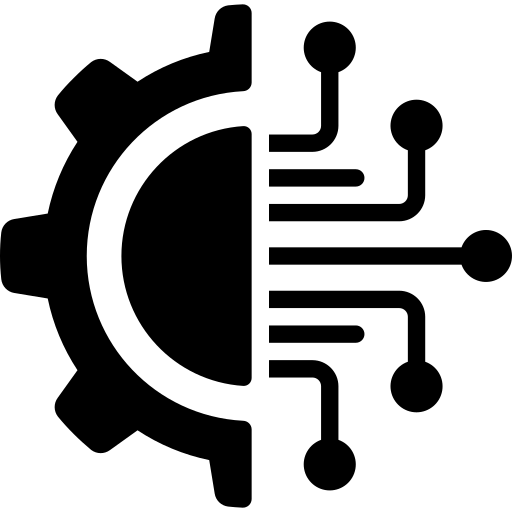
\includegraphics[scale=0.175]{semigear}
\end{figure}

Note : the secrets library is used, a library provided for cryptographic use.

\subsection{Key}

The key is made of three things :
\begin{itemize}
    \item A mixed set of chars (randomly swapped) coming from DEFAULT\_CHARSET defined in params.py, which the message should limit to 
          (chars not in this set will not be usable in the message !).
    \item A key field, which is the "seed" that will be used for Hasse's algorithm.
    \item A split char, that will be used to split the message and noise. If present in the message, it is removed.
    \item A set of "null chars", that should NOT be used in the message (doing so will stop the program).
\end{itemize}

\subsubsection{Key generation}

\begin{itemize}
    \item The unused chars defined in params.py are splited in 3 : one char is defined as the split char, and the rest is randomly 
          distributed among null chars and charset. The split char is part of the charset.
    \item The 'key' field is filled with secret's function token\_hex (actually makes a $2 \times$nbytes long hex number).
\end{itemize}

\subsubsection{Key storage}

Keys are nothing more than dictionaries (content described just above). They are stored as json with additional informations. Each 
key is stored in one file, named after the fingerprint (SHA256) of the key (in json format).

\begin{figure}[H]
    
\includegraphics[scale=0.08]{warning}
    The key is stored IN CLEAR, meaning anyone having access to it can decrypt any message encrypted with it !
\end{figure}

However, it is possible to only store a random string, thereafter called salt, which combined with a password and hashed, can be used 
as a seed to regenerate the key each time it is neeeded. This is recommendend, especially if your system and backups are not encrypted !

Please note that the key is not stored in encrypted form, but rather regenerated each times. Its hash is used to determine if the password 
is valid.


\subsection{Message encryption}
\begin{itemize}
    \item The message is splited in blocks (of 4096 chars by default). 
    \item Noise is added to the begining and the end of the message as well as between all the blocks, using the spliting char as a separator. 
          This is to make each encryption of the message unique (see the section below) and cryptanalysis difficult/confusing.
    \item Hasse's algorithm is applied to generate a sequence (as long as the message) of numbers modulus the size of the charset. If 
          the sequence is too short (compared to the message size), it is repeated.
    \item Each character $i$ is swapped with the character $i + key[i]$ modulus the size of the charset. Plus, there are between 1 and 45\% 
          of chance that a null char would be added at each character encoding. (this percentage is "decided" at each message encryption)
    \item Optionally, the enciphered message can be encoded in base64 (so that the message can be transmitted via channels that does not 
          support UTF-8).
\end{itemize}

\subsection{Message decryption}
\begin{itemize}
    \item Null chars are removed.
    \item Each character $i$ is swapped with the character $i - key[i]$ (+ the size of the charset, if the result is negative).
    \item The noise is removed using the split char. (by ignoring odd blocks)
\end{itemize}